% ISC 2026 submission draft for Project A.
% This source follows the official LNCS template supplied with the project.
% Replace the author and affiliation placeholders before submission.
\documentclass[runningheads]{llncs}
\usepackage[T1]{fontenc}
\usepackage{graphicx}
\usepackage{booktabs}
\usepackage{amsmath}
\usepackage{amssymb}
\usepackage{url}
\usepackage{xcolor}
\usepackage{microtype}

\begin{document}

\title{Missing Does Not Mean Zero: Reporting-Aware Forecasting for Rotating Disease Surveillance}
\titlerunning{Reporting-Aware Forecasting for Disease Surveillance}

\author{Nhi-Yen Nguyen-Huynh\inst{1,2} \and
Nguyen Quoc Khanh Le\inst{2,4}\thanks{Corresponding author: Nguyen Quoc Khanh Le. Tel.: +886-02-27361661 \#7174; E-mail: khanhlee@tmu.edu.tw.}}
\authorrunning{N.-Y. Nguyen-Huynh and N.Q.K. Le}
\institute{University of Economics and Law, Vietnam National University Ho Chi Minh City, Ho Chi Minh City, Vietnam \\
AIBioMed Lab, Taipei Medical University, Taipei, Taiwan \\
International Ph.D. Program in Medicine, College of Medicine, Taipei Medical University, Taipei, Taiwan \\
In-Service Master Program in Artificial Intelligence in Medicine, College of Medicine, Taipei Medical University, Taipei, Taiwan}

\maketitle
\footnotetext{Best Student Paper Award eligibility: Eligible.}

\begin{abstract}
Weekly disease surveillance data often omit conditions from a bulletin because of a reporting or ranking process, not because the observed count is zero. Treating such omissions as zeros can therefore distort both historical trajectories and forecast evaluation. This paper presents a reporting-aware forecasting protocol for a district-week-condition panel extracted from 164 weekly surveillance bulletins in Khyber Pakhtunkhwa, Pakistan. The protocol makes four observation states explicit, compares zero-fill with reporting-aware reconstruction, and evaluates forecasts under rolling-origin splits with a locked final test block. In addition to last-value, seasonal, and moving-average baselines, we study count models, tree-based models, uncertainty intervals, observation-process diagnostics, and controlled missingness stress tests. The panel contains 115,456 cells, including 43,384 structurally unreported cells and 12,248 district or cell non-reporting cells. The missingness audit is MNAR-like under a predictive diagnostic, with AUROC 0.805 using recent volume and 0.925 after adding condition fixed effects. Reporting-aware preprocessing improves the rotating-condition stress test for several baselines, while the effect is small for complete conditions. A multi-mechanism stress test shows a larger advantage as injected historical missingness increases, reaching 8.51 to 12.40 MAE points at 80\% missingness and horizon four. Temporal generalization and feature ablations show that the gain depends on the reporting regime and on which observation features are available. The study supports a narrow but practical conclusion: missingness should be modeled as part of the observation process, and absence in a surveillance table should not be silently interpreted as zero incidence.

\keywords{disease surveillance \and missing data \and time-series forecasting \and observation process \and rolling-origin evaluation}
\end{abstract}

\section{Introduction}

Public-health surveillance systems frequently publish compact weekly summaries rather than a complete measurement for every disease and reporting unit. A condition may be absent from a bulletin because it was not among the ranked items, because a district did not report that condition, or because the source recorded a non-response. These cases have different meanings from an observed count of zero. Nevertheless, a common preprocessing shortcut maps every absent value to zero. The shortcut is computationally convenient, but it can manufacture artificial declines, change lag features, and reward a forecasting method for reproducing the reporting process rather than the underlying signal.

This paper studies that problem in a reproducible district-week-condition setting. The central question is not whether one model is universally best. It is whether forecast validity changes when the observation process is represented explicitly. We construct a complete panel, label four observation states, and compare a zero-filled representation with a reporting-aware reconstruction. The comparison is performed under chronological rolling-origin evaluation, with the final 20 origins held out as a locked test block. The same panel is also used for mechanism diagnostics, uncertainty assessment, district heterogeneity, and controlled stress tests.

The contributions are fourfold. First, we provide an auditable panel construction that separates structural non-reporting, district or cell non-reporting, reported-but-not-recorded values, and observed numeric counts. Second, we evaluate reporting-aware preprocessing across baseline and machine-learning forecasters without using future information. Third, we quantify how reporting rotation changes the apparent disease trajectory and forecast uncertainty. Fourth, we test robustness across temporal blocks, feature ablations, and three injected missingness mechanisms at rates up to 80\%.

The paper is organized as follows. Section~\ref{sec:related} reviews relevant forecasting and missingness perspectives. Section~\ref{sec:data} describes the surveillance panel and observation states. Section~\ref{sec:method} presents reconstruction, features, models, and evaluation. Section~\ref{sec:protocol} defines the experiments. Section~\ref{sec:results} reports the findings, followed by discussion and limitations in Section~\ref{sec:discussion} and conclusions in Section~\ref{sec:conclusion}.

\section{Related Work}\label{sec:related}

Missing-data methodology distinguishes mechanisms such as missing completely at random, missing at random, and missing not at random, but these labels are assumptions about a data-generating and observation process rather than properties that can be established from a single diagnostic. Classical treatments emphasize that the estimand and the observation mechanism must be considered together~\cite{little2019statistical,rubin1987multiple}. In time series, intermittent observations also create a temporal censoring problem: the length and pattern of a reporting gap can carry information about when a series will reappear.

Forecasting research provides strong baselines for autoregressive and seasonal problems, and emphasizes rolling evaluation when the deployment setting is temporal~\cite{hyndman2021forecasting}. Tree-based learners can capture nonlinear lag interactions, while count models such as Poisson and negative-binomial regression are natural candidates for nonnegative case counts~\cite{ke2017lightgbm}. However, most forecasting comparisons assume that a missing value has already been resolved and do not treat the reporting process as an object of evaluation.

Uncertainty methods provide a related validity check. Quantile regression and conformal prediction can construct predictive intervals under suitable exchangeability or calibration conditions~\cite{romano2019conformal,vovk2005algorithmic}. Their empirical coverage can nevertheless be affected by selection and by long reporting gaps. Our work therefore combines point forecasting with an observation-process audit and reports interval coverage only for the combinations with sufficient calibration data.

\section{Data and Observation States}\label{sec:data}

\subsection{Surveillance panel}

The source is a public release of district-week notifiable infectious-disease surveillance data for Khyber Pakhtunkhwa, Pakistan, covering 164 bulletin weeks and 44 reporting units. The long-format file contains 59,824 source rows and 16 conditions. We construct the Cartesian product of weeks, districts, and conditions, yielding 115,456 panel cells. The panel is joined to the condition-presence matrix that records whether a condition was included in a week's bulletin.

\begin{table}
\caption{Audited panel composition.}\label{tab:data}
\centering
\begin{tabular}{lr}
\toprule
Quantity & Count \\
\midrule
Source rows & 59,824 \\
Bulletin weeks & 164 \\
Reporting units & 44 \\
Conditions & 16 \\
Panel cells & 115,456 \\
Structurally unreported & 43,384 \\
District or cell unreported & 12,248 \\
Reported but non-recorded & 291 \\
\bottomrule
\end{tabular}
\end{table}

Six conditions are present in every bulletin and form the complete confirmatory set: AD\_noncholera, Malaria, ILI, ALRI\_u5, Bloody\_diarrhoea, and Typhoid. The remaining conditions are rotating and are used as an exploratory stress-test set. This separation is important because a complete condition does not contain condition-level structural absence, so a large zero-fill contrast should not be expected for that group.

\subsection{Four observation states}

For each panel cell, we define an observation state. An observed target is a numeric count in a condition and district that is present in the source row. A true reported zero is an observed numeric zero. A district or cell non-report is a condition that is listed for the week but has no district-cell row. A structural non-report is a condition that is absent from that week's ranked condition columns. A source row with a missing count is retained as reported-but-not-recorded. These states are kept in the data and are never silently collapsed into a single missing-value flag. Let $M_{dct}\in\{0,1\}$ denote whether district $d$, condition $c$, and week $t$ has an observed numeric target, and let $P_{ct}$ denote condition presence in the bulletin. The state encoder used by the pipeline is
\begin{equation}
S_{dct}=\begin{cases} \mathrm{positive/zero}, & M_{dct}=1,\\ \mathrm{reported\text{-}NR}, & P_{ct}=1,\ \text{row present},\ M_{dct}=0,\\ \mathrm{cell\text{-}unreported}, & P_{ct}=1,\ \text{row absent},\\ \mathrm{structural\text{-}unreported}, & P_{ct}=0.\end{cases}
\end{equation}
The panel explicitly retains both $M_{dct}$ and $P_{ct}$, so structural absence is not confused with a reported zero.

\begin{figure}
\centering
\includegraphics[width=\textwidth]{Pipline.png}
\caption{Reporting-aware forecasting pipeline. The central panel preserves observation states before the two preprocessing alternatives are compared. Forecasting and uncertainty are evaluated on rolling origins, while observation-process analyses form a complementary diagnostic branch.}\label{fig:pipeline}
\end{figure}

\begin{figure}
\centering
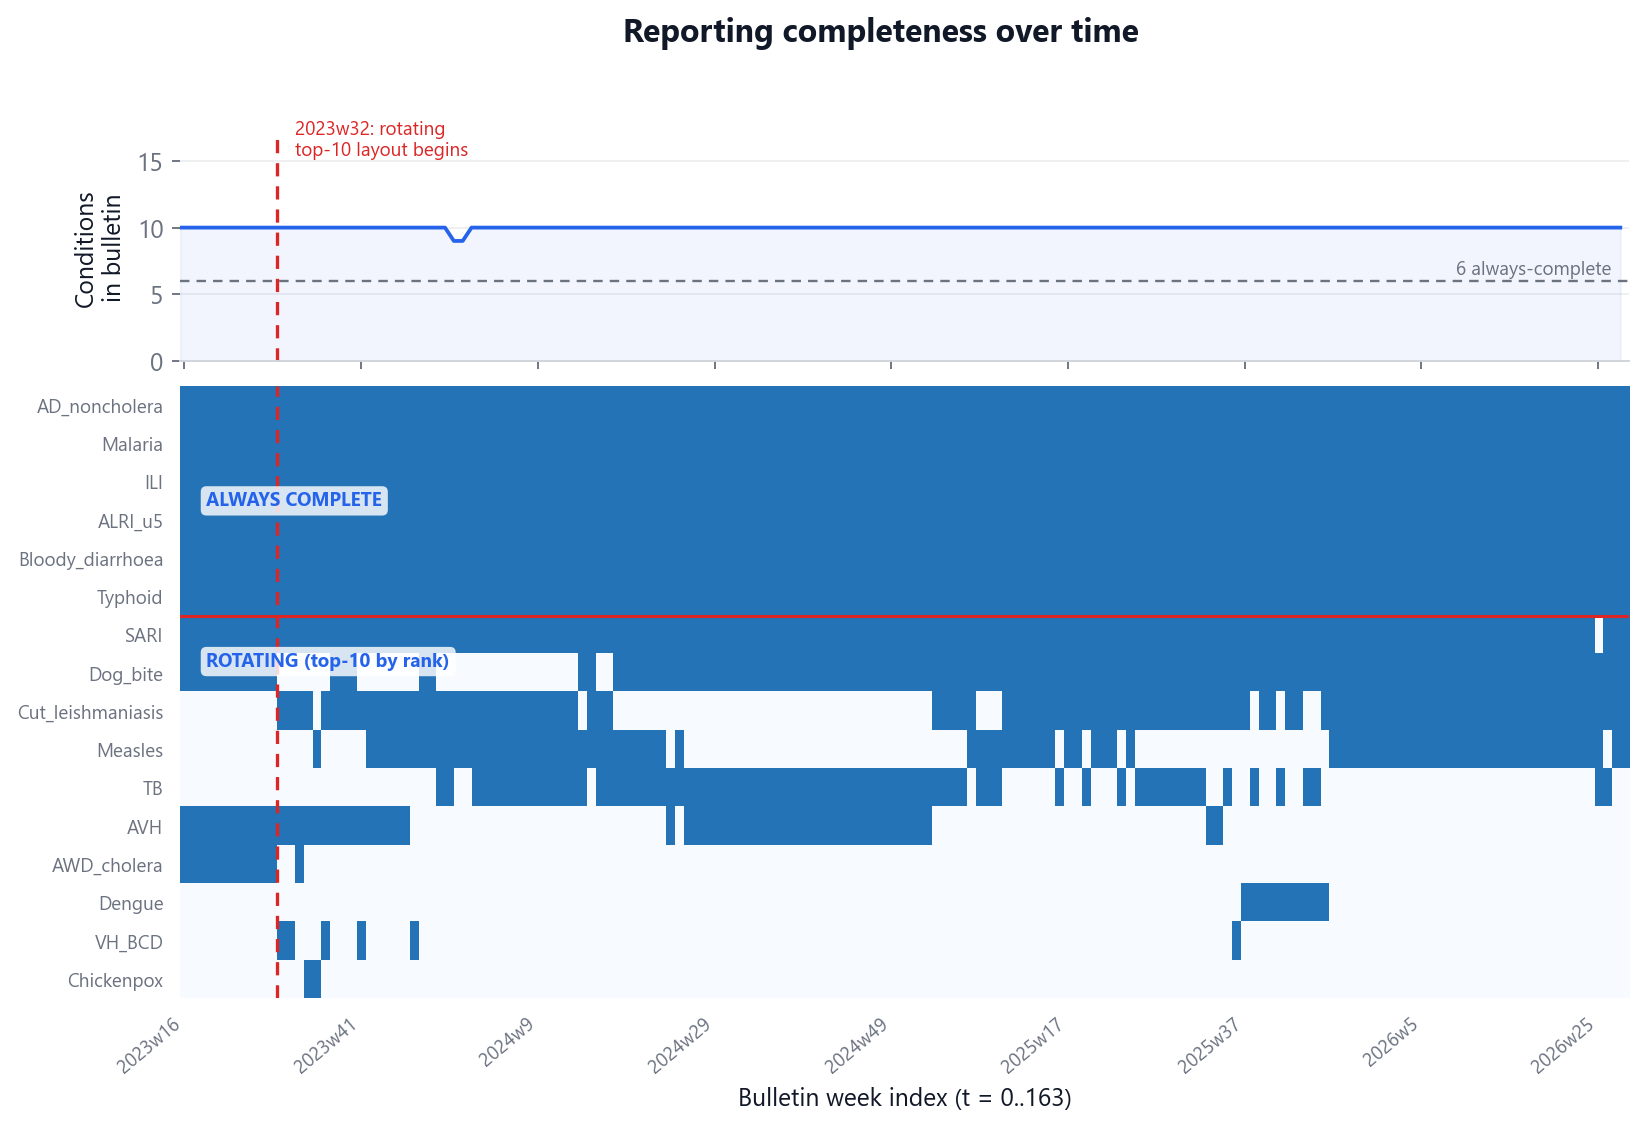
\includegraphics[width=\textwidth]{figure2_reporting_timeline.png}
\caption{Reporting completeness over time. Navy indicates conditions present in the bulletin and the lighter field indicates periods in which rotating conditions are not listed. The palette is intentionally redundant with the labels so the figure remains interpretable in grayscale.}\label{fig:timeline}
\end{figure}

\section{Methodology}\label{sec:method}

\subsection{Preprocessing alternatives}

For zero-fill, an unobserved historical value is replaced by zero. For reporting-aware reconstruction, the historical value is carried forward from the most recent observed value for the same condition and district. We implement this as a censoring-aware operator
\begin{equation}
\tilde{y}^{(a)}_{dct}=\begin{cases}y_{dct},&M_{dct}=1,\\y_{dc\tau^*},&M_{dct}=0,\ \tau^*=\max\{\tau<t:M_{dc\tau}=1\},\\0,&\nexists\tau<t:M_{dc\tau}=1.\end{cases}
\end{equation}
The reconstruction is used only to form historical features. Evaluation targets remain the original observed counts, and predictions whose targets are not observed are excluded from the primary error metric. This design avoids treating an imputed target as ground truth.

\subsection{Features and forecasting models}

At each forecast origin $t$, the feature vector contains lags at 1, 2, 4, 8, and 12 weeks, a four-week mean, and sine and cosine seasonal terms:
\begin{equation}
\mathbf{x}_{dct}^{(m)}=[\tilde{y}^{(m)}_{dc,t-1},\tilde{y}^{(m)}_{dc,t-2},\tilde{y}^{(m)}_{dc,t-4},\tilde{y}^{(m)}_{dc,t-8},\tilde{y}^{(m)}_{dc,t-12},\overline{y}_{dc,t-4:t-1},\sin(2\pi t/52),\cos(2\pi t/52),\mathbf{z}_{dct}].
\end{equation}
Here $m\in\{0,a\}$ denotes zero-fill or aware reconstruction. The observation vector $\mathbf{z}_{dct}$ contains seen indicators for lag positions and the missing count in the preceding eight weeks. A separate reporting-propensity model uses train-only history to provide a mechanism-informed predictive feature. It is not interpreted as a causal effect estimate.

We evaluate last-value, seasonal-naive, and four-observation moving-average baselines. The extended model family includes ridge regression, log-ridge, Poisson and negative-binomial models, random forest, and LightGBM. The count models are treated as comparative statistical baselines because no population denominator is available for an incidence-rate offset.

\subsection{Evaluation metrics}

For observed targets, we report MAE and RMSE. Paired comparisons use the same district, origin, condition, horizon, and method under the two preprocessing alternatives. Bootstrap intervals resample at the appropriate cluster level when dependence is present. The paper focuses on paired differences and their uncertainty rather than presenting the metric definitions as a contribution.

\subsection{Observation-process diagnostics}

We fit a predictive presence diagnostic using recent reported volume and condition fixed effects:
\begin{equation}
\Pr(P_{ct}=1)=\operatorname{logit}^{-1}(\alpha+\beta\log(1+v_{c,t-1})+\gamma_c),
\end{equation}
where $v_{c,t-1}$ is recent reported volume. The result is described as MNAR-like because it is evidence of value-related selection in this data, not a proof of a universal missingness mechanism. A reappearance hazard analysis separates cross-sectional presence prediction from the temporal question of when a missing series returns. We also compare trajectory reconstructions for Measles and TB and evaluate uncertainty coverage by reporting stratum.

\section{Experimental Protocol}\label{sec:protocol}

All primary forecasts use chronological rolling origins. For origin $o$ and horizon $h$, the target is $y_{dc,o+h-1}$ and the training set satisfies $t<o$. The final 20 origins are locked before model fitting and are not used for feature selection, propensity fitting, or interval calibration. The minimum training history is 12 weeks and the evaluated horizons are 1, 2, and 4 weeks. The primary observed-target metric is therefore conditional on the target being recorded, which is stated explicitly in every result. For a stress-test mechanism $g$, injection rate $r$, and horizon $h$, our estimand is the paired degradation
\begin{equation}
\Delta_{g,r,h}=\sum_{d,c,o}w_{dco}\left[\left|y_{d,c,o+h-1}-\hat{y}^{(0,g,r)}_{dcoh}\right|-\left|y_{d,c,o+h-1}-\hat{y}^{(a,g,r)}_{dcoh}\right|\right],
\end{equation}
where $w_{dco}$ are normalized target-count weights. Positive values mean that zero-fill incurs greater error under the specified observation perturbation. Confidence intervals are obtained by resampling condition-district clusters rather than treating adjacent weekly predictions as independent.

The principal stress test injects missingness only into pre-test history while retaining the known target values. It compares MCAR sampling, contiguous outage blocks, and value-dependent censoring at 10\%, 20\%, 40\%, 60\%, and 80\%, with 20 repetitions per configuration. The study also evaluates temporal generalization at four historical block starts and performs an ablation of base lags, seen-lag indicators, missing-run length, and the full observation mask. Smoke tests verify panel integrity, chronological splitting, future-feature exclusion, exact injection counts, and untouched test masks before the full local runs.

\section{Results}\label{sec:results}

\subsection{Panel audit and missingness mechanism}

The four-state audit produced the panel composition in Table~\ref{tab:data}. The predictive presence diagnostic yielded a coefficient of 2.31 (95\% CI [1.81, 2.81], $p=6.1\times10^{-20}$). AUROC was 0.805 with recent volume alone and 0.925 after adding condition fixed effects. These values support a value-related selection signal in the reporting process, while not identifying a causal incidence model.

\subsection{Baseline forecasting}

On the locked final block, the pooled four-observation moving average was the strongest baseline. At horizon one, zero-fill and reporting-aware MAE were 30.1934 and 30.1703, respectively. At horizons two and four, the corresponding MAE values were 30.4764 versus 30.4514 and 31.7226 versus 31.6950. The contrast is small for the complete six-condition set. In the rotating-condition stress test, paired gains favored reporting-aware preprocessing by 0.167 MAE for last-value and 0.634 MAE for seasonal-naive at horizon one, with bootstrap intervals [0.057, 0.299] and [0.421, 0.876].

\begin{figure}
\centering
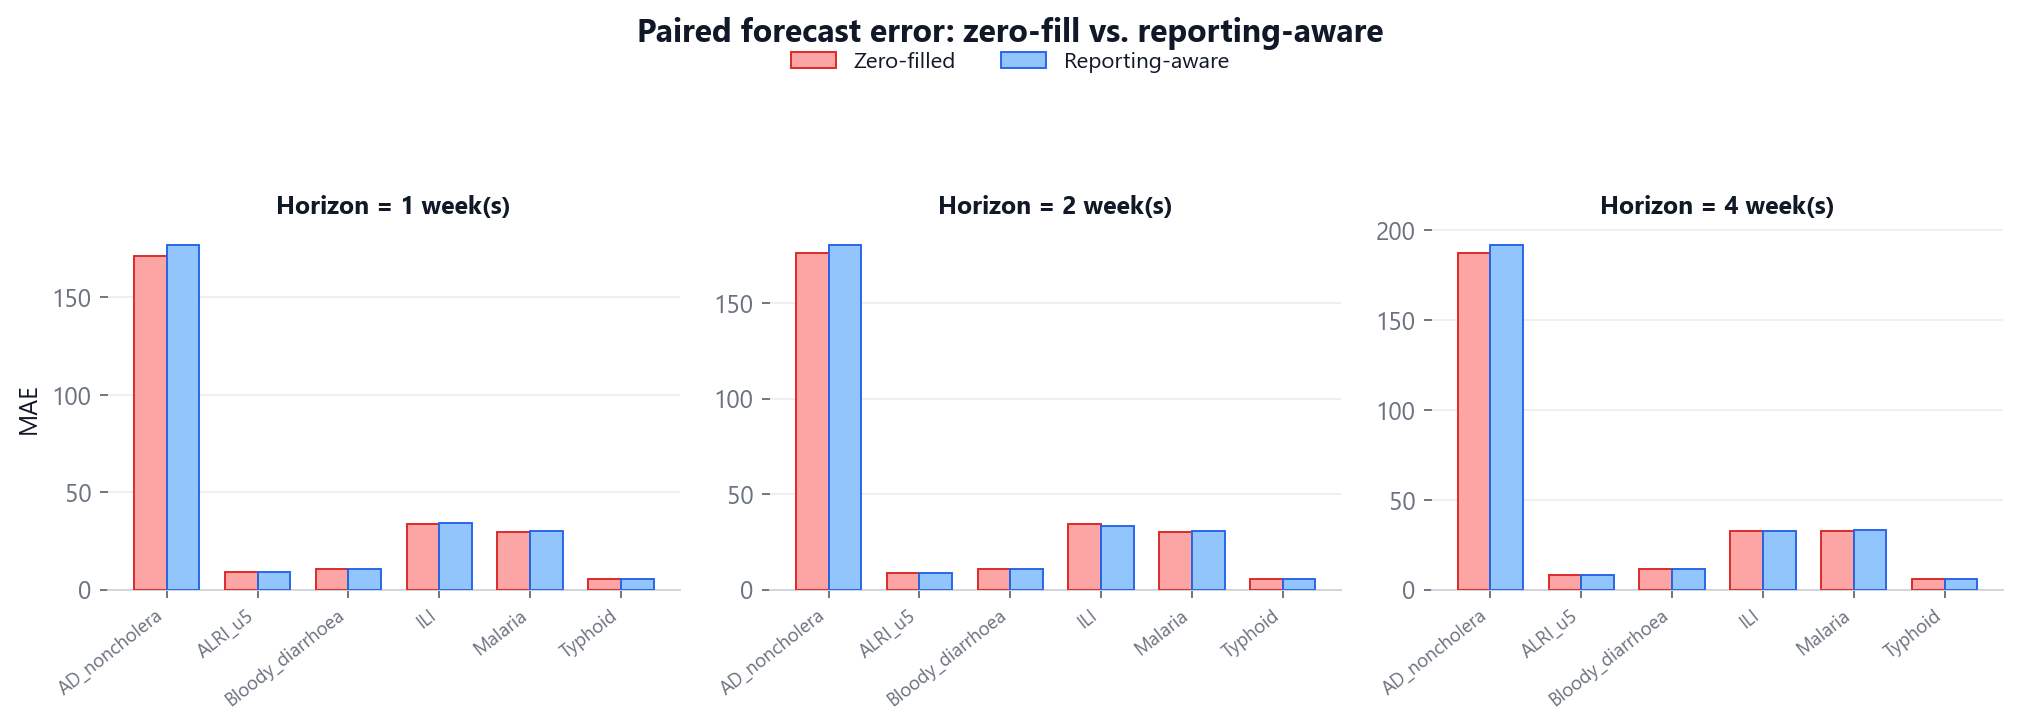
\includegraphics[width=\textwidth]{figure3_paired_errors.png}
\caption{Paired forecast error for the six complete conditions. Red and blue are reserved for zero-fill and reporting-aware preprocessing, respectively, and are paired with direct labels in the legend.}\label{fig:paired}
\end{figure}

\subsection{Trajectory distortion and uncertainty}

The trajectory case study makes the preprocessing difference visible. We quantify distortion on censored weeks with
\begin{equation}
D_c=\frac{1}{|\mathcal{C}_c|}\sum_{t\in\mathcal{C}_c}\frac{|\tilde{y}^{(0)}_{ct}-\tilde{y}^{(a)}_{ct}|}{\max(\tilde{y}^{(a)}_{ct},1)},\quad \mathcal{C}_c=\{t:P_{ct}=0\},
\end{equation}
and separately report the fraction of censored weeks with relative distortion above 25\%. The latter was 81.0\% for Measles and 66.3\% for TB. Empirical residual intervals under-covered: average coverage was approximately 0.718--0.724 for nominal 80\% intervals and 0.823--0.833 for nominal 90\% intervals. Quantile and split-conformal intervals were closer to nominal for combinations with enough training and calibration data; 30 condition-horizon-mode combinations were skipped rather than assigned an unsupported coverage value. For a calibration residual quantile $q_{\alpha}$, the split-conformal interval used in the pipeline is $[\max(0,\hat{y}-q_{\alpha}),\hat{y}+q_{\alpha}]$, with $q_{\alpha}$ estimated without the locked test block.

\begin{figure}
\centering
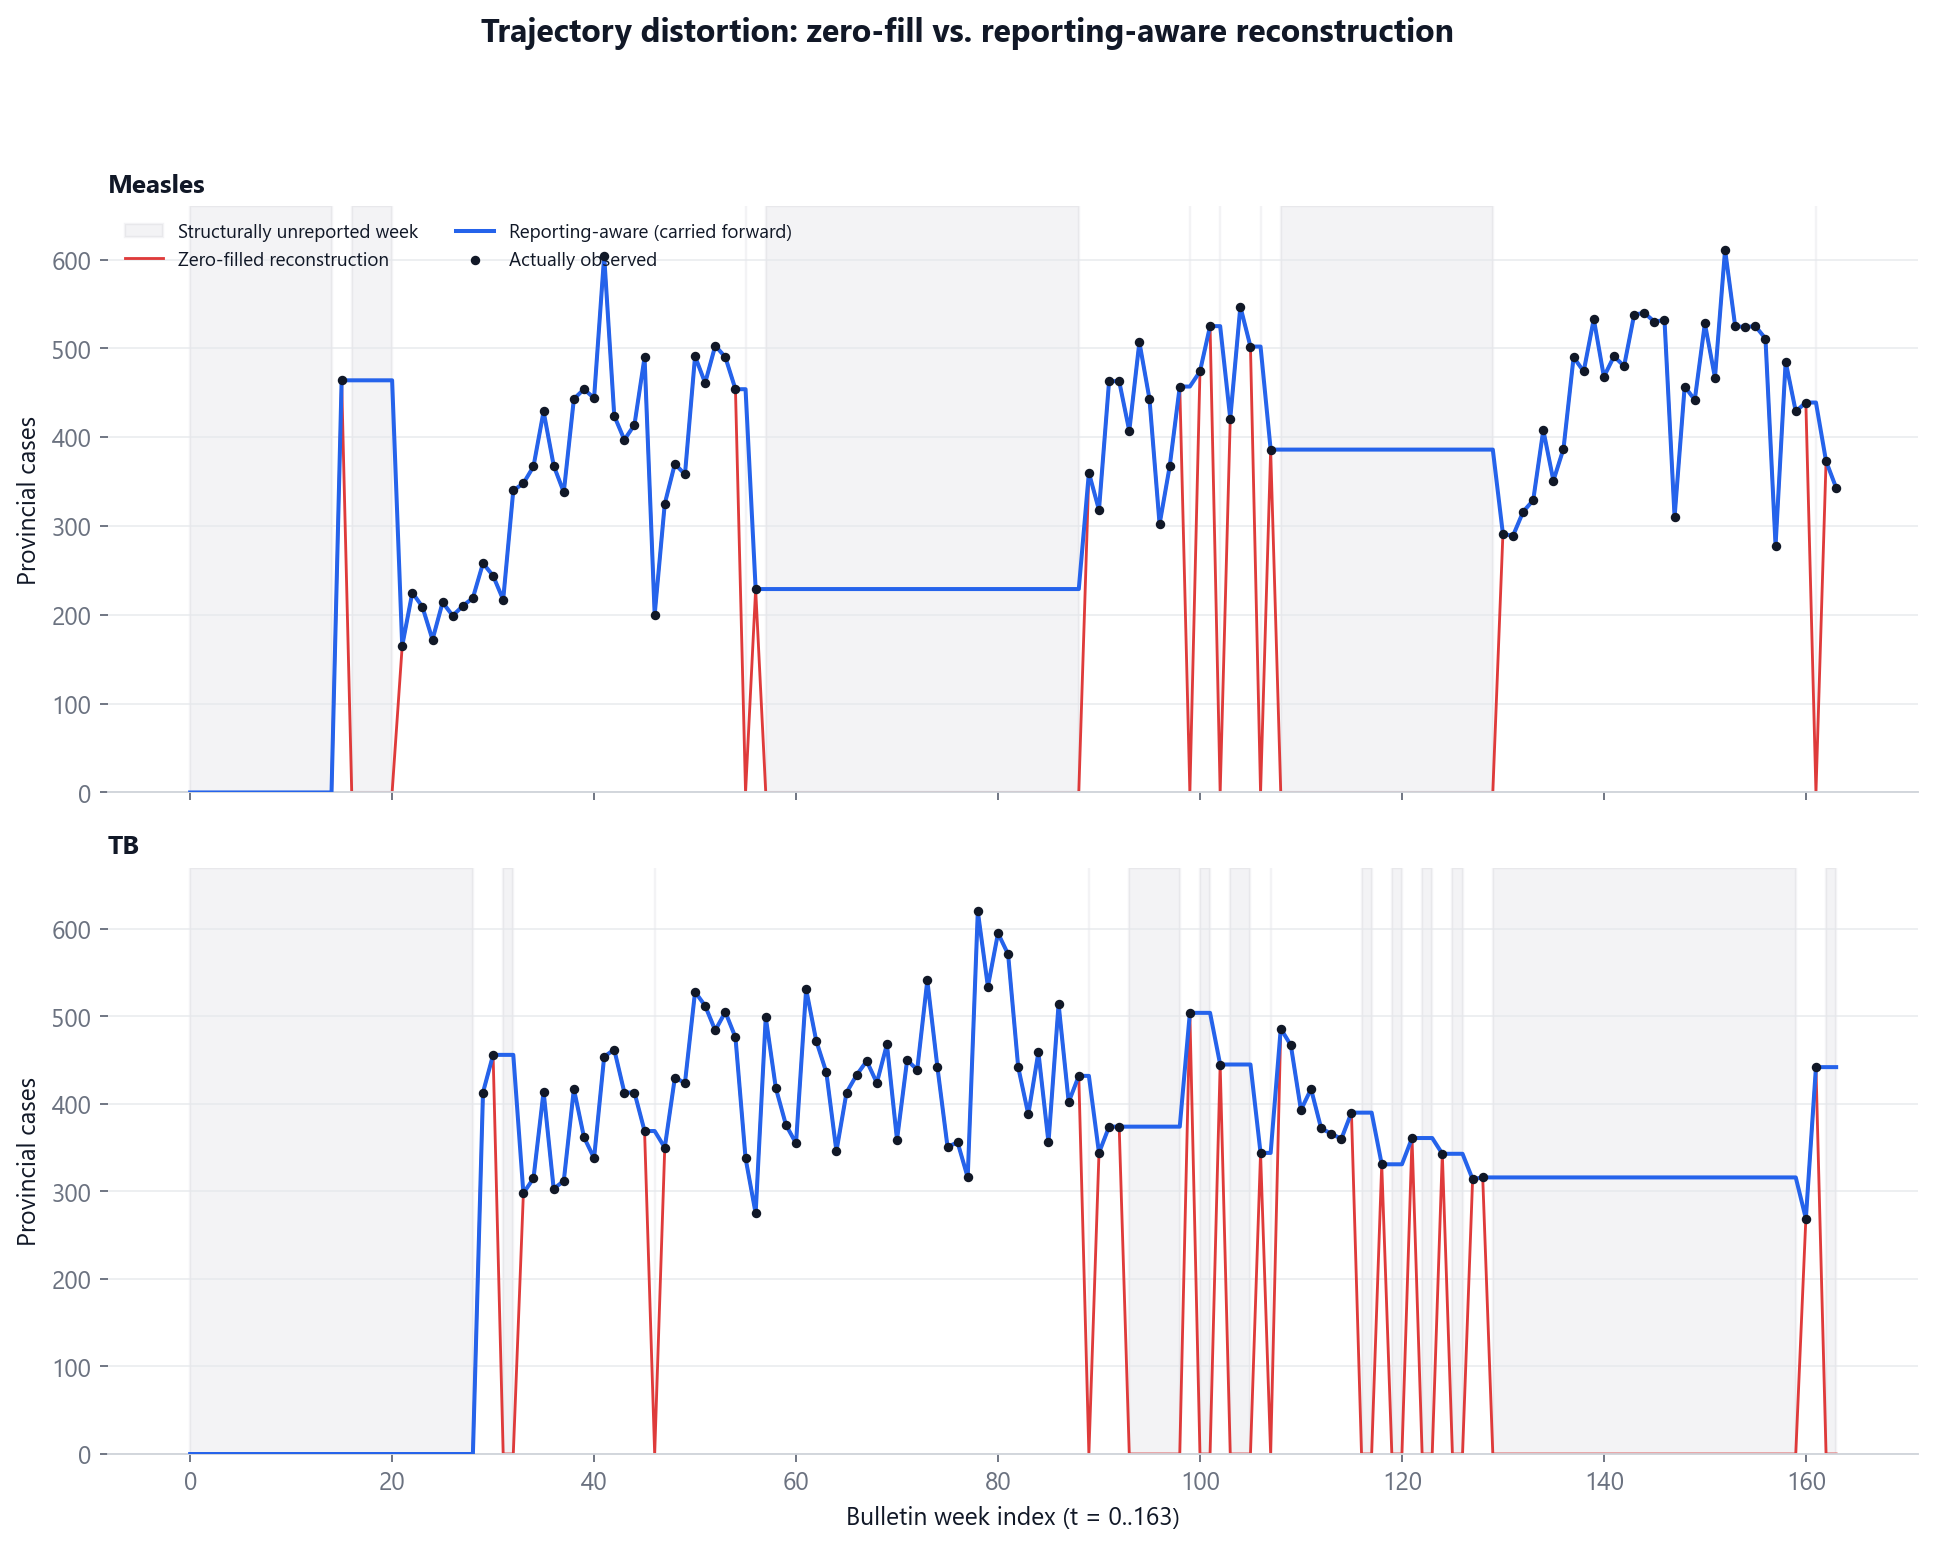
\includegraphics[width=\textwidth]{figure5_trajectory_distortion.png}
\caption{Trajectory distortion for two rotating conditions. The red reconstruction treats an unobserved week as zero, whereas the teal reconstruction carries forward the last observed count. Shaded intervals mark structurally unreported weeks.}\label{fig:trajectory}
\end{figure}

\begin{table}
\caption{Multi-mechanism stress test at horizon four. Values are pooled MAE across 6 complete conditions, 44 districts, 20 repetitions, and the locked target origins.}\label{tab:stress}
\centering
\begin{tabular}{lrrrr}
\toprule
Mechanism & Rate & Zero-fill & Aware & $\Delta$ zero--aware (95\% CI) \\
\midrule
MCAR & 40\% & 65.47 & 59.46 & 6.01 [3.77, 8.64] \\
MCAR & 80\% & 72.24 & 60.41 & 11.83 [7.04, 17.22] \\
Block outage & 40\% & 66.05 & 59.98 & 6.07 [3.39, 9.63] \\
Block outage & 80\% & 71.81 & 63.30 & 8.51 [4.58, 13.26] \\
Value-dependent & 40\% & 64.05 & 59.18 & 4.87 [2.69, 7.55] \\
Value-dependent & 80\% & 72.38 & 59.98 & 12.40 [7.56, 18.46] \\
\bottomrule
\end{tabular}
\end{table}

\subsection{Stress test, temporal generalization, and ablation}

The multi-mechanism stress test in Table~\ref{tab:stress} consistently favors reporting-aware reconstruction and shows a larger gap as historical missingness increases. This is controlled simulation evidence: the target values are known and only the historical observation mask is perturbed. It is not a causal estimate of disease incidence.

Temporal generalization is conditional rather than universal. With the full mask, aware MAE improved at several historical blocks, including horizon four at $t=80$ (39.08 versus 39.79), but zero-fill was lower at other blocks such as horizon one at $t=100$ (50.46 versus 51.08). The ablation gives a similar message. For reporting-aware forecasts, base-lag MAE was 44.36, 45.55, and 47.93 at horizons 1, 2, and 4. Adding seen-lag indicators yielded 44.32, 45.46, and 47.86; missing-run length yielded 44.21, 45.29, and 47.84; and the full mask yielded 44.33, 45.18, and 47.71. No single component dominates every horizon, but observation features provide measurable conditional information.

\subsection{Additional model and robustness findings}

LightGBM produced the strongest condition-specific results in the extended family, for example MAE 5.051 at horizon one for Measles and 5.653 for Typhoid. Propensity used as a train-only feature improved the paired estimate in all six evaluated condition groups and was stable across the tested seeds. The same quantity used as a simple inverse-propensity loss weight did not improve the complete group and harmed the rotating group. A hazard model achieved AUROC 0.815 for reappearance duration, compared with 0.545 for recent volume alone, based on 37 events in 623 person-period rows.

\section{Discussion and Limitations}\label{sec:discussion}

The results support a narrow methodological message. Reporting-aware preprocessing is most useful when the observation process creates genuine rotation or long reporting gaps. The complete-condition baseline contrast is small because those conditions are present throughout the bulletin sequence. Conversely, trajectory distortion and the multi-mechanism stress test show that zero-filling can become increasingly consequential as missingness and forecast horizon grow. The temporal block results caution against presenting the method as universally superior. A more defensible interpretation is that the observation process should be audited and exposed to the model when it is predictive of the recorded value.

Several limitations constrain the claims. The data provide counts but no population denominator, so the analysis is not an incidence-rate study. The source covers 164 weeks from one surveillance system, and external validation on another region or release is not available. The primary metric is evaluated on observed targets, which is appropriate for reproducible benchmarking but does not identify the unobserved counterfactual burden. The hazard analysis has few reappearance events, and the propensity and IPW analyses are protocol-specific predictive comparisons rather than causal estimators. Controlled missingness experiments retain known targets and therefore quantify sensitivity to the injected mask, not the true disease process. Finally, the reported runtime is an engineering benchmark on the current implementation and hardware, not a guarantee of deployment performance.

\section{Conclusion}\label{sec:conclusion}

This paper presented an observation-aware forecasting protocol for rotating disease surveillance. An explicit four-state panel audit identified substantial structural non-reporting and a measurable value-related selection signal. Reporting-aware reconstruction reduced forecast error in rotating-condition baselines and remained advantageous across MCAR, block, and value-dependent stress tests, especially at high missingness and longer horizons. Temporal generalization and feature ablation showed that the gain is conditional on the reporting regime and on the information carried by observation features. The practical conclusion is simple: a missing surveillance entry is an observation-state event, not automatically a zero. Preserving that distinction improves the validity of both analysis and forecast evaluation.

\begin{credits}
\subsubsection{Acknowledgments} The authors thank the data contributors and the organizers of ISC 2026. Funding and institutional details should be completed before submission.

\subsubsection{Competing Interests} The authors have no competing interests to declare that are relevant to the content of this paper.
\end{credits}

\begin{thebibliography}{8}
\bibitem{little2019statistical}
Little, R.J.A., Rubin, D.B.: Statistical Analysis with Missing Data, 3rd edn. Wiley, Hoboken (2019)

\bibitem{rubin1987multiple}
Rubin, D.B.: Multiple Imputation for Nonresponse in Surveys. Wiley, New York (1987)

\bibitem{hyndman2021forecasting}
Hyndman, R.J., Athanasopoulos, G.: Forecasting: Principles and Practice, 3rd edn. OTexts, Melbourne (2021)

\bibitem{ke2017lightgbm}
Ke, G., Meng, Q., Finley, T., Wang, T., Chen, W., Ma, W., Ye, Q., Liu, T.-Y.: LightGBM: A highly efficient gradient boosting decision tree. In: Advances in Neural Information Processing Systems, vol. 30 (2017)

\bibitem{romano2019conformal}
Romano, Y., Patterson, E., Cand\`es, E.J.: Conformalized quantile regression. In: Advances in Neural Information Processing Systems, vol. 32 (2019)

\bibitem{vovk2005algorithmic}
Vovk, V., Gammerman, A., Shafer, G.: Algorithmic Learning in a Random World. Springer, New York (2005)

\bibitem{nawab2026surveillance}
Nawab, S., Khan, G., Abbas, A., et al.: District-week notifiable infectious disease surveillance data for Khyber Pakhtunkhwa, Pakistan, 2023--2026. Mendeley Data, version 1 (2026). \doi{10.17632/9yzvfgrhkt.1}

\bibitem{isc2026}
International Computer Symposium 2026: Call for papers and submission instructions. \url{https://www.ics2026.ntub.edu.tw/call-for-paper/}
\end{thebibliography}

\end{document}
